\section{Results}
\subsection{Calibration}
Due to \hl{small defects in }the construction and hardware of the antenna, the pointing of the antenna doesn't always line up with the target. It is therefore necessary to calibrate it before pointing at distant objects. The Sun \st{being} \hl{is} the strongest discrete radio source in the sky \cite{burke_introduction_2013}, mostly due to black body radiation\hl{, and is therefore an ideal target for the calibration}.
By configuring the antenna to point towards Sun, using its actual coordinates, and scanning the surrounding area in Az/Alt coordinates, the maximum average measured power gives the real position of the Sun in the specific antenna coordinates. The measured power and a linear interpolation of those values shown in \autoref{fig:calibration_contour} gives a correction \hl{to the pointing} of
\begin{equation}
    \textrm{Az: } -5.25^\circ \qquad \textrm{Alt: } -2.70^\circ \\
\end{equation}
\begin{figure}[htbp]
    \centering
    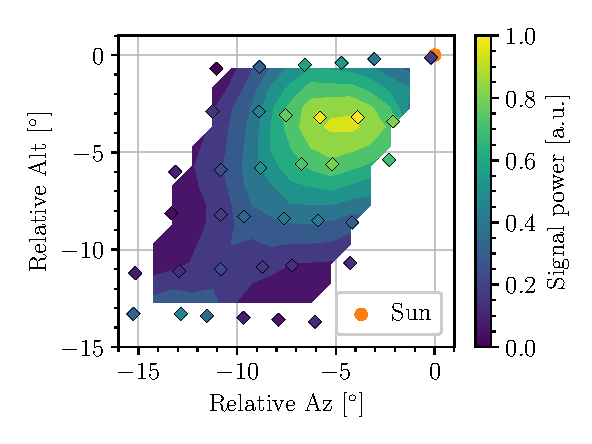
\includegraphics[scale=1]{figures/calibration_contour.pdf}
    \caption{Interpolation of signal power measured in the proximity of the sun. }
    \label{fig:calibration_contour}
\end{figure}

\subsection{Distinguishing signal and noise}
The signal must be cleaned of the [] noise.
To this end, measures were taken with the telescope pointed towards a nearby building, in order for the spectrum to only contain the noise (same noise which will then appear in actual measures).

Measure BM building, measure actual H21 source, divide actual by noise to extract the signal from noise, apply some filter and voilà, a nice signal

\subsection{Velocity field of the Milky Way}
Probing arms of milky way

Talk about orientation (i.e. sky visible at measuring time), correct angular momentum?
